\documentclass{article}

\usepackage[spanish, es-nodecimaldot]{babel}
\usepackage[most]{tcolorbox}
\usepackage[letterpaper,top=2cm,bottom=2cm,left=3cm,right=3cm,marginparwidth=1.75cm]{geometry}

\usepackage{amsmath}
\usepackage{graphicx}
\usepackage{caption}
\usepackage{subcaption}
\usepackage{booktabs}
\usepackage[colorlinks=true, allcolors=blue]{hyperref}

\newtcolorbox[auto counter]{exercise}[1][]{
    colback=blue!5!white,
    colframe=blue!75!black,
    fonttitle=\bfseries,
    title=Ejercicio \thetcbcounter,
    #1
}

\title{Aprendizaje no supervisado:\\ segmentación de nubes de puntos LiDAR con k-means y DBSCAN}
\author{Juan José Cabrera y Arturo Gil}

\begin{document}
\maketitle

\section{Introducción}
Hasta ahora, todo el aprendizaje que hemos hecho ha sido \textbf{supervisado}: disponíamos de ejemplos $x$ \textbf{y de su respuesta correcta} $y$. El \textbf{aprendizaje no supervisado} trabaja únicamente con $X$: el algoritmo debe descubrir por sí mismo la estructura que hay en los datos. En este ámbito, la tarea más habitual y conocida se denomina \textbf{agrupamiento} (\textit{clustering}): búsqueda de grupos de ejemplos parecidos entre sí.

En esta práctica agruparemos los datos de un sensor LiDAR. Este tipo de sensor está instalado en una gran cantidad de coches autónomos y muchos robots. ¿Para qué se instala este sensor?: un coche que circula necesita saber qué parte de lo que ve es \textbf{suelo} y qué \textbf{objetos} (coches, peatones, farolas, muros) tiene alrededor. En este contexto, resulta inviable etiquetar a mano cada punto de cada nube: un solo barrido tiene más de cien mil puntos y el sensor produce diez por segundo. ¿Hasta dónde podemos llegar \textbf{sin etiquetas}?

\begin{tcolorbox}[colback=yellow!8!white, colframe=orange!70!black, title=\textbf{Las etiquetas sólo sirven para medir}]
Nuestros barridos tienen etiquetas puestas a mano, pero \textbf{los algoritmos que programaremos en esta práctica no las verán nunca}: usaremos técnicas que agrupan solamente utilizando las coordenadas cartesianas de los puntos o bien otras características de los puntos. Las etiquetas se usarán, \emph{después}, para medir la precisión del proceso de \textit{clustering}. En un problema real no existen estas etiquetas, y la única forma de juzgar un agrupamiento es \textbf{dibujarlo y observarlo}. Por esta razón, durante esta práctica usaremos la librería \texttt{open3d} para juzgar el resultado.
\end{tcolorbox}

\subsection{El sensor LiDAR}
Un LiDAR (\textit{Light Detection and Ranging}) emite pulsos de luz láser en diferentes direcciones. El sensor mide el \textbf{tiempo de vuelo} desde que la luz sale del sensor, impacta sobre un objeto y se refleja de vuelta sobre el sensor: como la luz viaja a una velocidad conocida ($3\cdot 10^8$ $m/s$, en el vacío), el tiempo de vuelo permite deducir la distancia al obstáculo. Conociendo además la dirección en la que salió el pulso, cada eco es un \textbf{punto 3D}. Usaremos barridos reales del conjunto de datos \textbf{KITTI}\footnote{A. Geiger, P. Lenz y R. Urtasun, \textit{Are we ready for autonomous driving? The KITTI vision benchmark suite}, CVPR, 2012. Licencia CC BY-NC-SA 3.0.}, grabados en Karlsruhe con un Velodyne HDL-64E montado en el techo de un coche. Las características de este sensor son:
\begin{itemize}
    \item \textbf{64 láseres} apilados verticalmente que giran 360\textdegree{} diez veces por segundo. Cada láser describe un círculo sobre el suelo: por eso las nubes se ven como \textbf{anillos} concéntricos.
    \item La densidad de puntos \textbf{decae con la distancia}: los objetos cercanos tienen miles de puntos y los lejanos, unos pocos.
    \item Ejes del sensor: $x$ hacia \textbf{delante} del coche, $y$ hacia la \textbf{izquierda} y $z$ hacia \textbf{arriba}. El sensor va a 1{,}73\,m del suelo, así que el suelo está en torno a $z \approx -1{,}7$\,m.
    \item Cada punto guarda también la \textbf{intensidad} del eco, entre 0 y 1: las superficies brillantes (matrículas, señales, marcas viales) devuelven más intensidad de luz.
\end{itemize}
Un barrido se guarda en un fichero \texttt{.bin} que no es más que una ristra de números \texttt{float32}, cuatro por cada punto: $x, y, z$, intensidad. Sus etiquetas son las de \textbf{SemanticKITTI}\footnote{J. Behley et al., \textit{SemanticKITTI: A Dataset for Semantic Scene Understanding of LiDAR Sequences}, ICCV, 2019. Licencia CC BY-NC-SA 4.0.}: un fichero \texttt{.label} con un entero por punto que dice su \textbf{clase} (calzada, acera, coche, edificio, vegetación\dots) y, en los objetos, su \textbf{instancia} (qué coche concreto es).

\subsection{Materiales}
Trabajaremos en el directorio \texttt{practice\_unsupervised\_learning\_lidar} del repositorio Intro2AI (\url{https://github.com/4rtur1t0/Intro2AI}). Instale \texttt{open3d} si lo necesita: \texttt{pip install open3d}. El directorio contiene:
\begin{itemize}
    \item \texttt{data/}: dos barridos con sus etiquetas. El principal, \texttt{kitti\_00\_001560}, es un cruce de calles de una zona residencial, con coches aparcados, edificios y árboles. El otro, \texttt{kitti\_08\_003880}, es para el apartado opcional.
    \item \texttt{lidar/nube.py}: lectura, recorte, colores y visualización \textbf{(ejercicio 1)}.
    \item \texttt{lidar/kmeans.py}: k-means desde cero \textbf{(ejercicio 2)}.
    \item \texttt{lidar/caracteristicas.py}: características geométricas de cada punto, ya programadas \textbf{(ejercicio 3)}.
    \item \texttt{lidar/suelo.py}: qué puntos son suelo según las etiquetas y las medidas de acierto, ya programado.
    \item \texttt{1\_visualizar\_main.py}, \dots, \texttt{4\_dbscan\_main.py}: un programa por ejercicio.
\end{itemize}
Los programas se ejecutan desde dentro del directorio (\texttt{python 1\_visualizar\_main.py}). Las partes que deben completarse están marcadas con \texttt{EJERCICIO: SE DEBE COMPLETAR EL CÓDIGO POR EL ESTUDIANTE} y lanzan \texttt{NotImplementedError} mientras no se completen. Cada ventana de \texttt{open3d} detiene el programa hasta que se cierra. Ratón: el botón izquierdo gira, la rueda acerca y \texttt{Ctrl}+botón izquierdo desplaza; las teclas \texttt{+} y \texttt{-} cambian el tamaño de los puntos.

\begin{tcolorbox}[colback=yellow!8!white, colframe=orange!70!black, title=\textbf{Antes de comenzar}]
Asegúrate de que tu editor de python está configurado correctamente:
\begin{itemize}
\item El intérprete de python debe apuntar al entorno virtual de las prácticas \texttt{venvAI}.
\item Usa el gestor de \texttt{git} para obtener la última versión del repositorio de prácticas.
\end{itemize}
\end{tcolorbox}


\section{Leer y ver un barrido}
Lea la nube con
\begin{verbatim}
    nube = np.fromfile(ruta, dtype=np.float32)
    nube = np.reshape(nube, [-1, 4])
\end{verbatim}
\texttt{np.fromfile} devuelve todos los números seguidos en un vector; \texttt{reshape} con $-1$ los coloca en filas de cuatro y calcula él solo cuántas filas salen.

\begin{exercise}\label{ej:visualizar}
Complete \texttt{cargar\_nube} y \texttt{a\_open3d} en \texttt{lidar/nube.py} y los huecos de \texttt{1\_visualizar\_main.py}:
\begin{enumerate}
    \item Calcule el \textbf{número de puntos} del barrido. Debe obtener \textbf{122\,485}.
    \item Visualice la nube en \texttt{open3d} \textbf{coloreada por la intensidad} (columna 3). La función \texttt{colores\_por\_valor} ya convierte un valor por punto en un color.
\end{enumerate}
El programa termina mostrando la nube \textbf{coloreada por clase} con las etiquetas de SemanticKITTI (figura~\ref{fig:barrido}) y una tabla con las clases presentes: calzada (33{,}7\,\%), edificio (17{,}5\,\%), acera (15{,}4\,\%), vegetación (12{,}5\,\%), coche (10{,}5\,\%)\dots
\end{exercise}

\begin{figure}[h]
\centering
\begin{subfigure}{0.48\textwidth}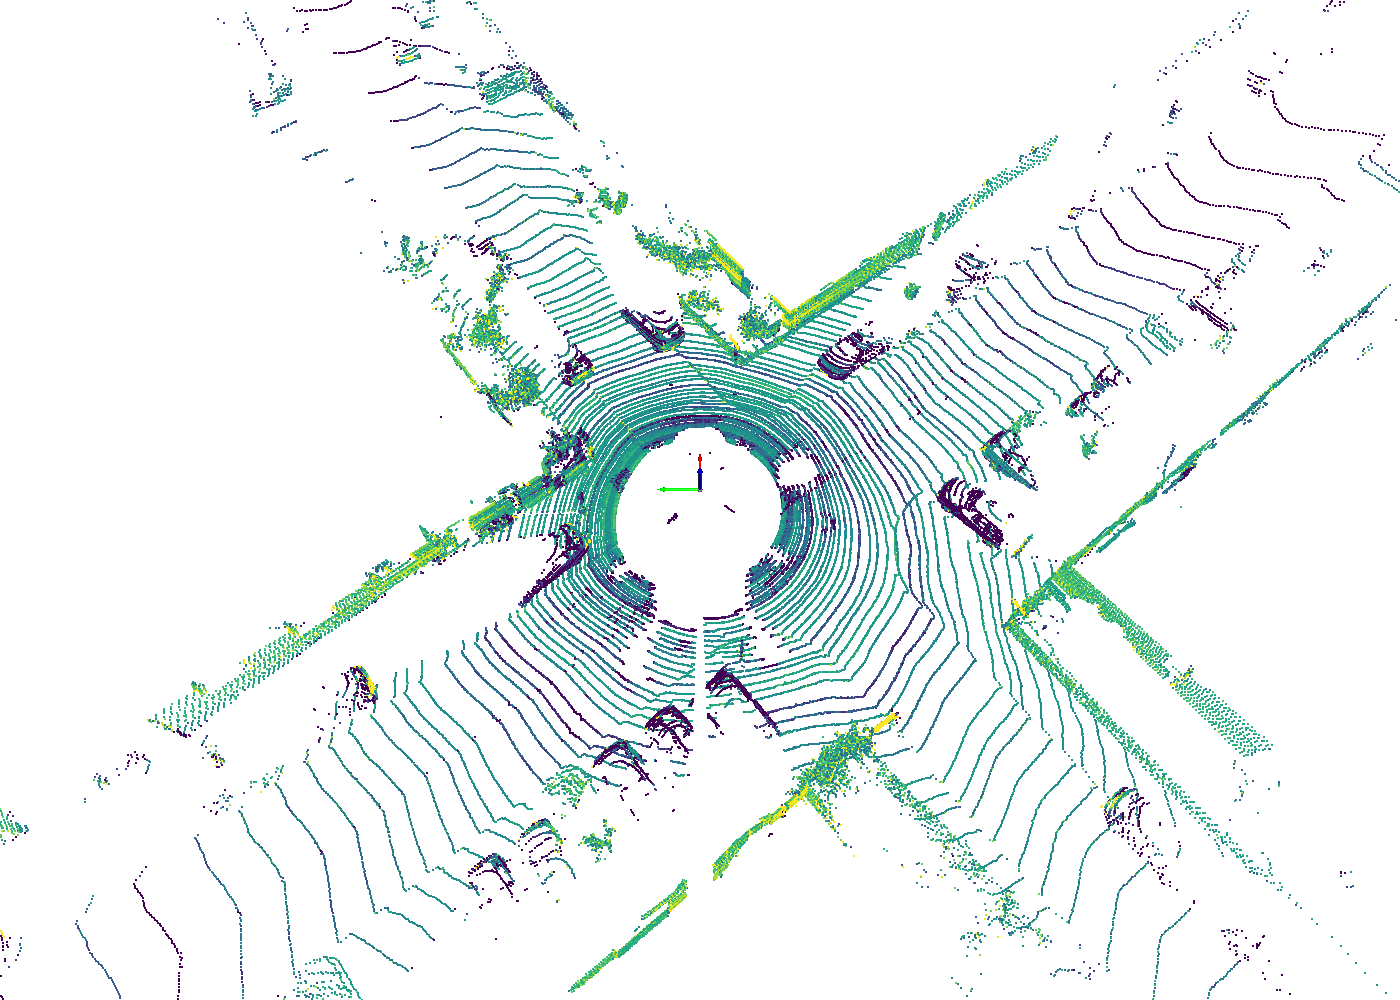
\includegraphics[width=\textwidth]{figures/ej1_intensidad.png}\caption{Color = intensidad.}\end{subfigure}
\begin{subfigure}{0.48\textwidth}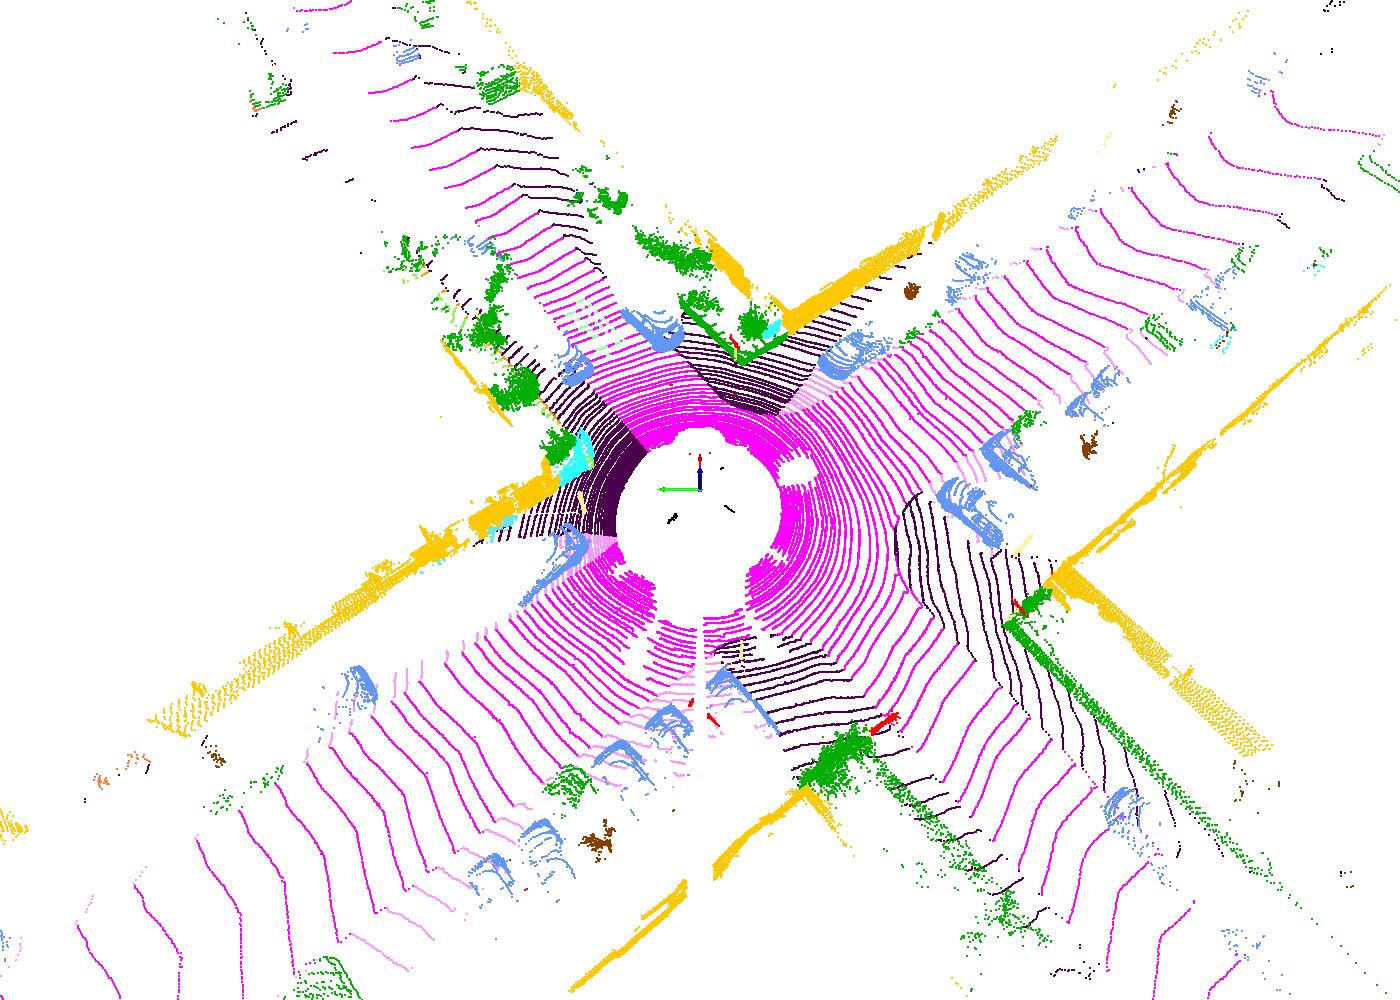
\includegraphics[width=\textwidth]{figures/ej1_clases.png}\caption{Color = clase: calzada en magenta, acera en morado, coches en azul, edificios en amarillo, vegetación en verde.}\end{subfigure}
\caption{El barrido 1560 de la secuencia 00, visto desde arriba con el coche avanzando hacia la parte superior de la imagen. Los ejes en el centro marcan el sensor (rojo $x$, verde $y$, azul $z$).}
\label{fig:barrido}
\end{figure}


\section{k-means desde cero}
k-means busca $k$ puntos, los \textbf{centroides}, que representen bien a los datos, y repite dos pasos hasta que se estabiliza:
\begin{enumerate}
    \item \textbf{Asignación}: cada punto se asigna al centroide más cercano.
    \item \textbf{Actualización}: cada centroide se mueve a la \textbf{media} de los puntos que se le han asignado.
\end{enumerate}
Lo que el algoritmo hace disminuir en cada iteración es la \textbf{inercia} total $J$, definida como la suma de las distancias al cuadrado de cada punto $x_i$ a su centroide $c_{j(i)}$:
\[
J = \sum_{i=1}^{N} \lVert x_i - c_{j(i)} \rVert^2 .
\]

\begin{exercise}\label{ej:kmeans}
Complete \texttt{asignar}, \texttt{actualizar}, \texttt{inercia} y \texttt{kmeans} en \texttt{lidar/kmeans.py} usando \texttt{numpy}. No recorra los puntos uno a uno con un bucle: con cien mil puntos sería muy lento; recorra los $k$ centroides y opere con todos los puntos a la vez.

Ejecute \texttt{2\_kmeans\_main.py}. Agrupa las coordenadas $(x, y, z)$ del recorte de 40\,m $\times$ 40\,m alrededor del sensor (109\,994 puntos) en $k = 4$ grupos y compara su k-means con el de \texttt{scikit-learn} partiendo de los \textbf{mismos centroides iniciales}. Si su implementación es correcta, ambos deben dar la misma inercia (\textbf{4\,136\,190,7}), el mismo número de iteraciones (37) y el 100\,\% de etiquetas iguales. ¿Qué forma tienen los cuatro grupos que se ven en \texttt{open3d}? ¿Separan objetos o simplemente reparten el espacio? Pruebe a cambiar k=5, 6, 7 \ldots. ¿Qué observa?
\end{exercise}

Hemos podido implementar el algoritmo k-means con un resultado igual al muy probado algoritmo de la librería Scikit-learn. Sin embargo, \textbf{la agrupación de los puntos no nos proporciona ninguna información de provecho}: simplemente agrupa los puntos por cercanía, mientras minimiza la inercia total del conjunto. \textbf{Así pues, la posición del punto no es una característica de interés para poder agrupar los puntos en entidades con significado.
}


\section{Suelo frente al resto: la importancia de las características}
Probemos con la tarea más sencilla: separar la nube recortada en \textbf{dos} grupos, suelo y todo lo demás. Según las etiquetas proporcionadas por KITTI, el 57{,}1\,\% de sus puntos son suelo (calzada, acera, aparcamiento, terreno\dots). A continuación, voveremos a ejecutar el algoritmo k-means de la misma manera, pero cambiaremos la información de cada punto. El algoritmo será siempre el mismo, k-means con $k = 2$, pero a cada punto le asignaremos otra información.

\begin{tcolorbox}[colback=gray!5!white, colframe=gray!60!black, title=\textbf{Cómo se evalúa: matriz de confusión y métricas}]
k-means no sabe cuál de sus dos grupos es el suelo: para evaluar se toma la correspondencia grupo $\rightarrow$ clase que más puntos acierta, como se hace siempre al comparar un agrupamiento con etiquetas. Con el \textbf{suelo como clase positiva}, cada punto cae en una casilla de la \textbf{matriz de confusión}: \textbf{TP} (suelo predicho como suelo), \textbf{FN} (suelo predicho como objeto), \textbf{FP} (objeto predicho como suelo) y \textbf{TN} (objeto predicho como objeto). De ella salen las métricas estándar:
\begin{gather*}
\text{accuracy} = \frac{TP + TN}{N}, \qquad
\text{precision} = \frac{TP}{TP + FP}, \qquad
\text{recall} = \frac{TP}{TP + FN}, \\
\text{F1-score} = \frac{2 \cdot \text{precision} \cdot \text{recall}}{\text{precision} + \text{recall}} = \frac{2TP}{2TP+FP+FN}, \qquad
\text{IoU} = \frac{TP}{TP + FP + FN}.
\end{gather*}
La \textbf{precision} dice qué parte de lo que se predice suelo lo es de verdad; el \textbf{recall}, qué parte del suelo real se encuentra. El \textbf{F1-score} los resume con su media armónica, que solo es alta si \emph{ambos} lo son. El \textbf{IoU} (intersección sobre unión, o índice de Jaccard) es la métrica oficial de SemanticKITTI: el tamaño de lo que coincide entre predicción y etiqueta dividido por el tamaño total de las dos. Como en la práctica 3, la \textbf{accuracy} sola puede resultar engañosa cuando una clase es mucho más frecuente que la otra.
Como recordatorio, damos una definición formal de los anteriores parámetros y lo aplicamos al caso que nos ocupa:
\begin{itemize}
\item \textbf{Accuracy}: la proporción de todas las predicciones correctas sobre las clases (en nuestro caso, sobre suelo  y otros). \textbf{Útil}: cuando el dataset está equilibrado y las predicciones sobre ambas clases también son correctas. \textbf{Limitación}: en el caso en el que el dataset está desequilibrado.
\item \textbf{Precision}: la cantidad de predicciones positivas correctas (TP) sobre el total de predicciones positivas (TP+FP). En nuestro caso, este parámetro mide la cantidad de puntos que se han clasificado como suelo y eran realmente suelo (TP) sobre el total de puntos que se han clasificado como suelo (TP+FP). \textbf{Útil}: cuando la aparición de FP es costosa. En el caso que nos ocupa, si nuestro clasificador encuentra un FP, ¿qué ocurre?: hay un punto que se ha clasificado como ``suelo'' que intentará ser transitado por nuestro coche autónomo, cuando realmente ``no es suelo''. En definitiva, \textbf{la precisión indica cómo de fiables son los puntos que se han clasificado como suelo}.
\item \textbf{Recall}: se calcula como el número de casos positivos reales (TP) que logró detectar el modelo sobre el total de casos positivos que hay en el dataset (TP+FN). En nuestro caso, mide la capacidad del clasificador para encontrar elementos de tipo ``suelo'' de entre el total de puntos de suelo existentes en el dataset.
\item \textbf{IoU}: mide la ratio entre los TP sobre el total de positivos en el \textit{ground truth}. En esencia es un parámetro que considera la capacidad del modelo para generar TP y lo pondera con la cantidad de FP y FN que también genera el modelo.
\item \textbf{F1-score}: es la media harmónica entre precision y recall. Se utiliza para poder simplificar el problema y utilizar un único parámetro para comparar diferentes métodos de clasificación.
\end{itemize}
\end{tcolorbox}

\begin{tcolorbox}[colback=gray!5!white, colframe=gray!60!black, title=\textbf{Características geométricas (ya calculadas)}]
Para cada punto, la función \texttt{caracteristicas\_geometricas} toma sus vecinos a menos de 0{,}5\,m y calcula la matriz de covarianza $3 \times 3$ de sus coordenadas. Sus autovectores definen las direcciones en que se extiende el vecindario (es un PCA local) y sus autovalores $\lambda_1 \geq \lambda_2 \geq \lambda_3$, indican amplitud en cada una de esas direcciones. La \textbf{normal} $\mathbf{n}$ de la superficie es la dirección en la que el vecindario varía \emph{menos}, esto es, la dirección asociada a $\lambda_3$. De ahí salen dos números por punto:
\begin{itemize}
    \item \textbf{Verticalidad} $= 1 - |n_z|$: 0 en superficies horizontales (calzada, techo de un coche) y 1 en verticales (paredes, laterales de los coches, troncos).
    \item \textbf{Curvatura} $= \lambda_3 / (\lambda_1 + \lambda_2 + \lambda_3)$: 0 en superficies lisas y hasta $1/3$ en vecindarios desordenados (vegetación, esquinas).
\end{itemize}
Antes de agrupar, cada característica se \textbf{estandariza} (se le resta su media y se divide por su desviación típica). De esta manera, eliminamos la influencia de las unidades y problemas de convergencia debido a la función de distancia.
\end{tcolorbox}

\begin{exercise}\label{ej:suelo}
Complete los huecos de \texttt{3\_suelo\_main.py} y ejecútelo. 

En la primera parte del programa, se muestra el suelo con \texttt{open3d} según las etiquetas conocidas de KITTI (figura~\ref{fig:suelo}a). A continuación, se evalúa la clasificación usando una \textbf{referencia trivial}. Con esta clasificación trivial (que dice que todo es suelo): accuracy 57{,}1\,\%, precision 57{,}1\,\%, recall 100\,\% y F1-score 72{,}7\,\%. \textbf{Nótese que este resultado es importante}, pues establece un límite inferior de los resultados: si hacemos una clasificación arbitraria, el F1-score es del 70\% aproximadamente, debemos superar este resultado con cualquier otra clasificación que hagamos.


Para cada elección de atributos el programa imprime la matriz de confusión y las cinco métricas (tabla~\ref{tab:suelo}).
\begin{enumerate}
    \item[a)] Atributos $(x, y, z)$. Debe obtener una accuracy del \textbf{51{,}8\,\%}, \emph{peor} que la referencia trivial, y un F1-score del 50{,}2\,\%. Mire el resultado en \texttt{open3d}: ¿por dónde corta k-means la nube? ¿Por qué, si $x$ e $y$ varían en 40\,m y $z$ apenas en unos metros?
    \item[b)] Solo el atributo $z$ (cuidado: la matriz debe ser $N \times 1$, no un vector). Debe obtener un \textbf{recall del 100\,\%} pero una \textbf{precision del 79{,}8\,\%}: hay 15\,917 falsos positivos. Los centroides quedan en $z = -1{,}67$ y $z = -0{,}20$\,m. Calcule la \textbf{frontera} entre los dos grupos, la altura a partir de la cual un punto pasa de un grupo al otro ($-0{,}93$\,m). ¿Qué son esos falsos positivos, qué parte de los coches y de los muros acaba llamando ``suelo'' k-means? ¿Por qué?
    \item[c)] Mire primero en \texttt{open3d} la nube coloreada por verticalidad y por curvatura (figura~\ref{fig:caracteristicas}): ¿qué sale en rojo?, ¿dónde es alta la curvatura? Después construya la matriz con $z$, verticalidad y curvatura. Debe obtener una precision del \textbf{95{,}9\,\%} y un recall del \textbf{98{,}6\,\%} (F1-score 97{,}2\,\%, IoU 94{,}6\,\%). ¿Qué ha arreglado la verticalidad respecto al apartado b)? Por último, comente la línea que estandariza y vuelva a ejecutar: la precision baja al 88{,}1\,\% (F1-score 93{,}7\,\%). ¿Por qué? (Pista: la desviación típica de la $z$ es 0{,}75\,m y la de la curvatura, 0{,}05.)
\end{enumerate}
\end{exercise}

\begin{figure}[h]
\centering
\begin{subfigure}{0.24\textwidth}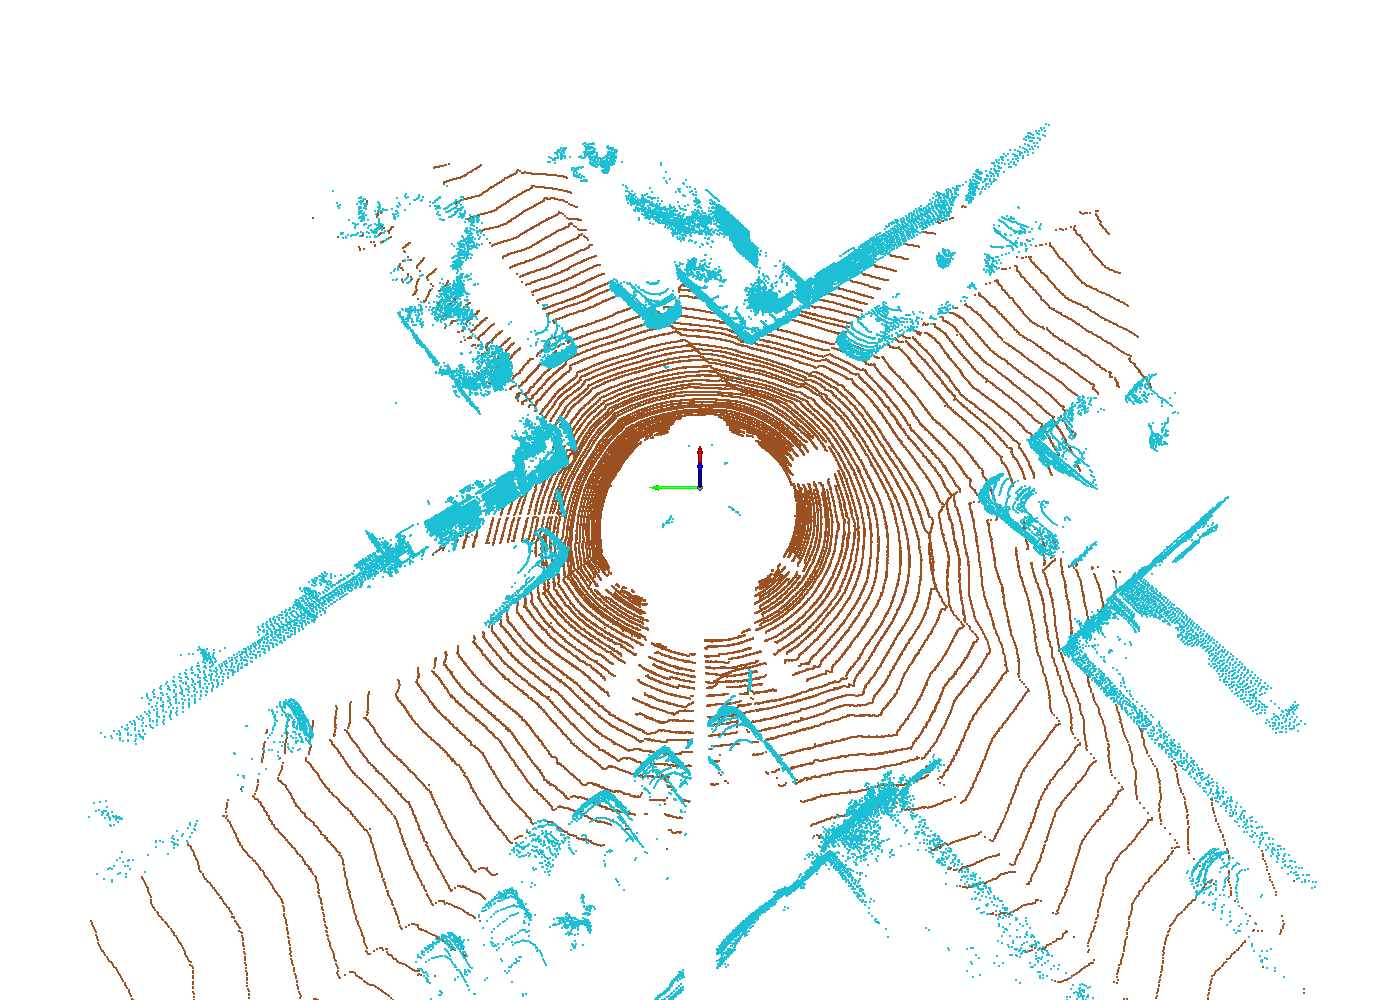
\includegraphics[width=\textwidth]{figures/ej3_referencia.png}\caption{Etiquetas.}\end{subfigure}
\begin{subfigure}{0.24\textwidth}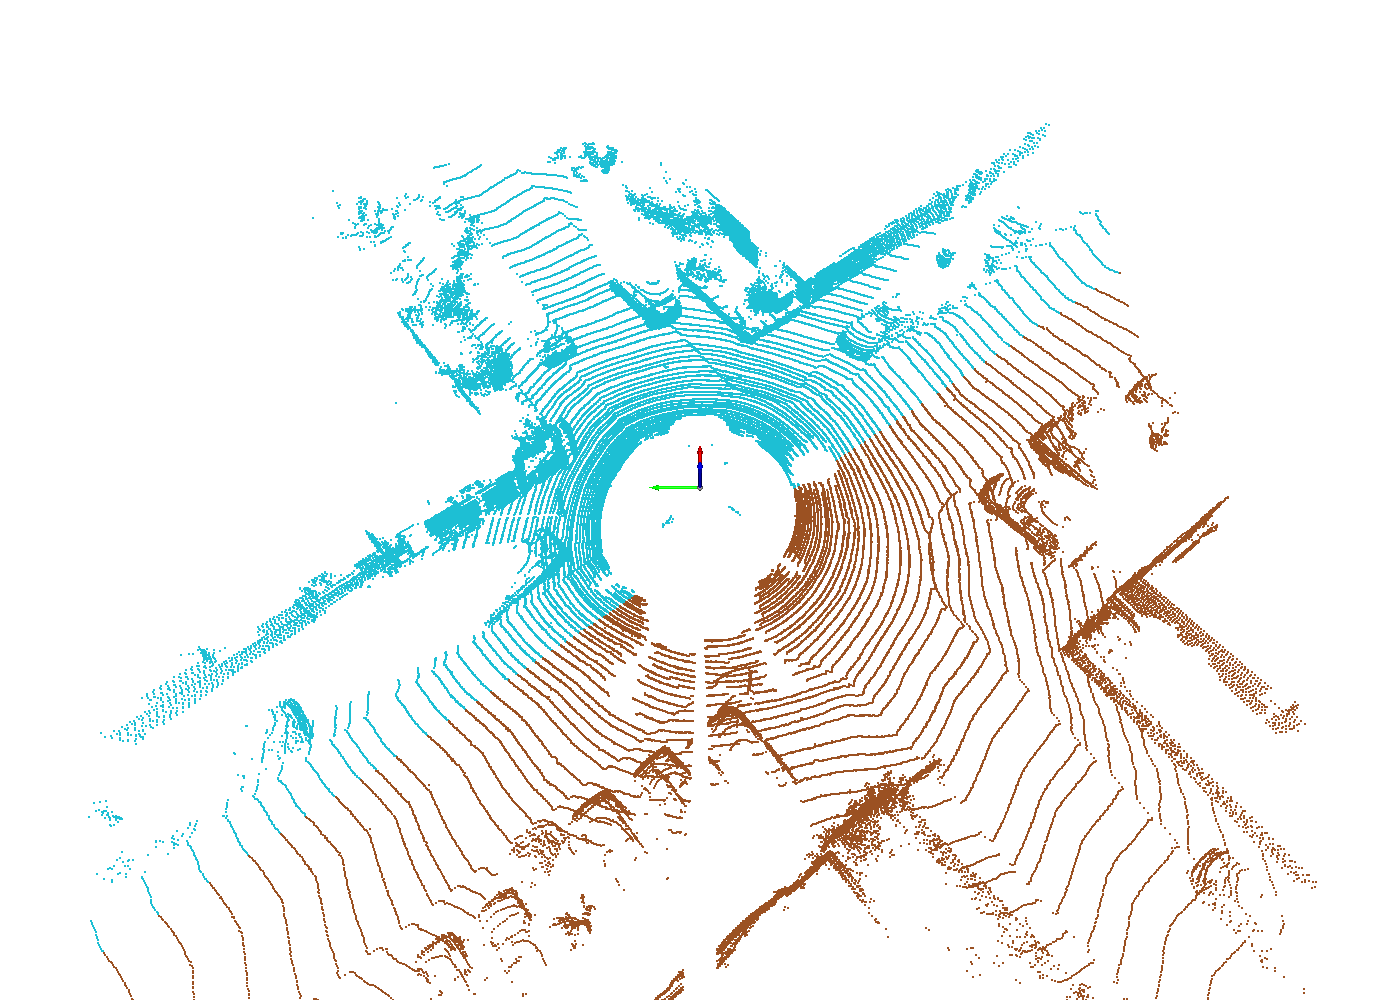
\includegraphics[width=\textwidth]{figures/ej3_xyz.png}\caption{$(x, y, z)$.}\end{subfigure}
\begin{subfigure}{0.24\textwidth}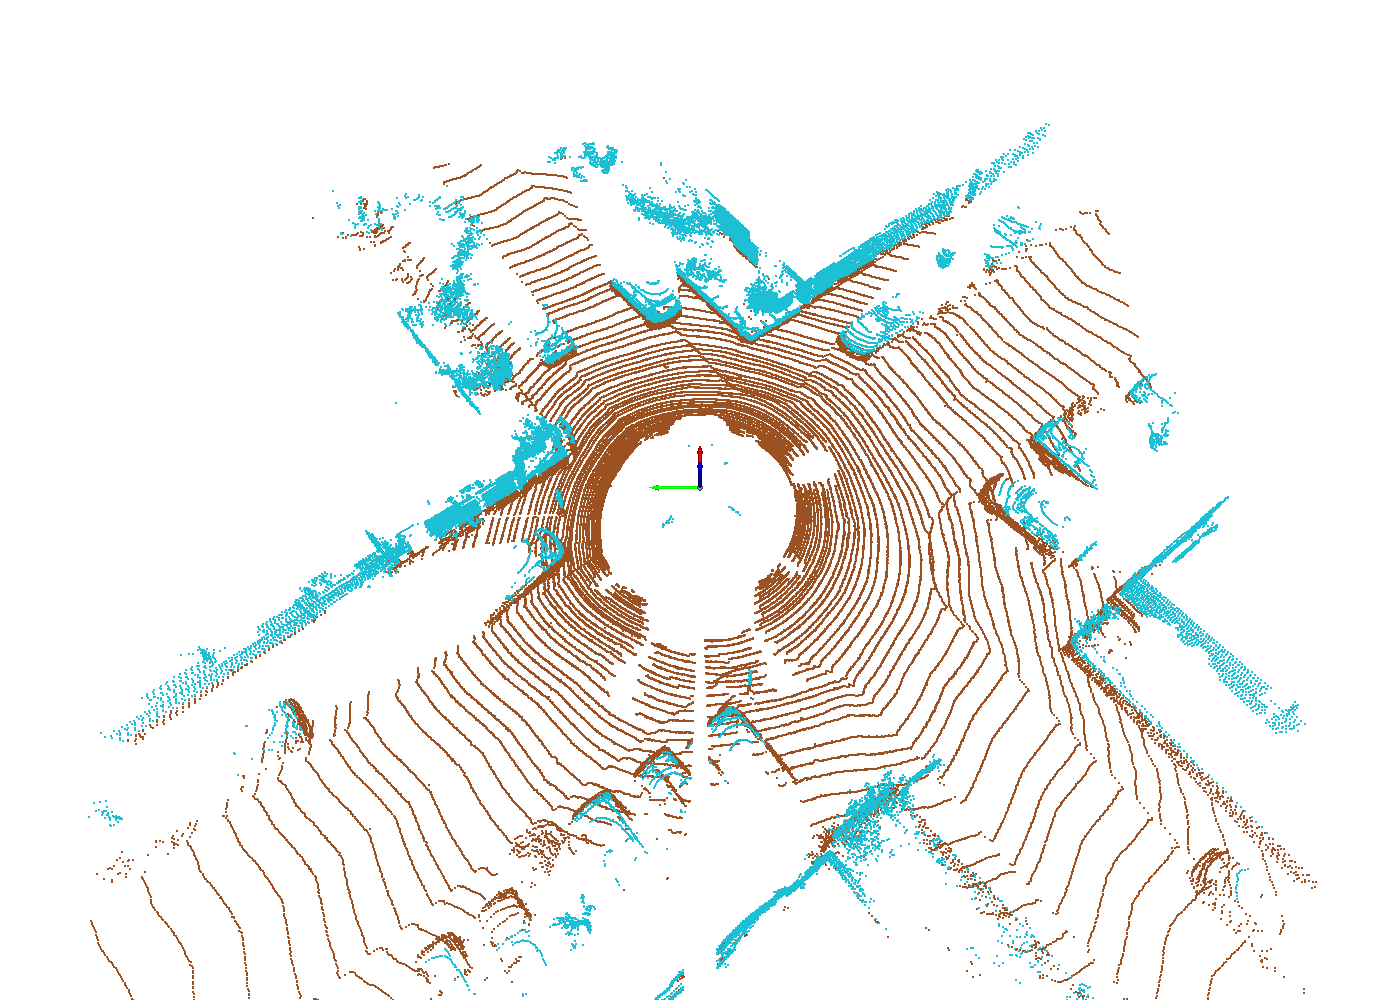
\includegraphics[width=\textwidth]{figures/ej3_z.png}\caption{$z$.}\end{subfigure}
\begin{subfigure}{0.24\textwidth}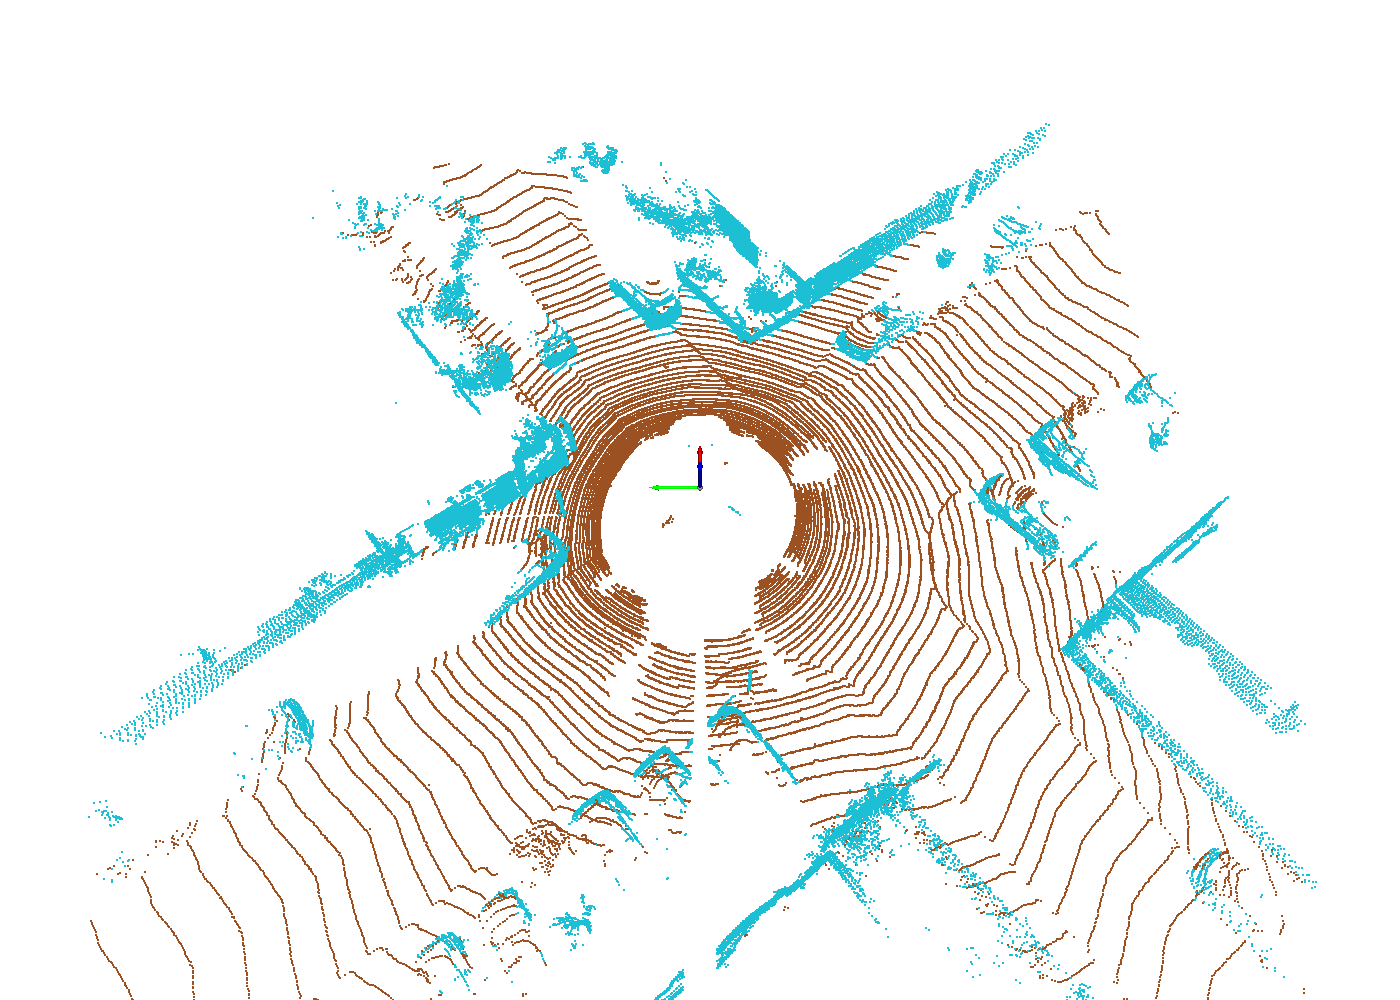
\includegraphics[width=\textwidth]{figures/ej3_geo.png}\caption{$z$ + geometría.}\end{subfigure}
\caption{Suelo (marrón) frente al resto (azul) en el recorte de 40\,m $\times$ 40\,m: (a) según las etiquetas; (b)--(d) según k-means con $k = 2$ y cada elección de atributos.}
\label{fig:suelo}
\end{figure}

\begin{figure}[h]
\centering
\begin{subfigure}{0.45\textwidth}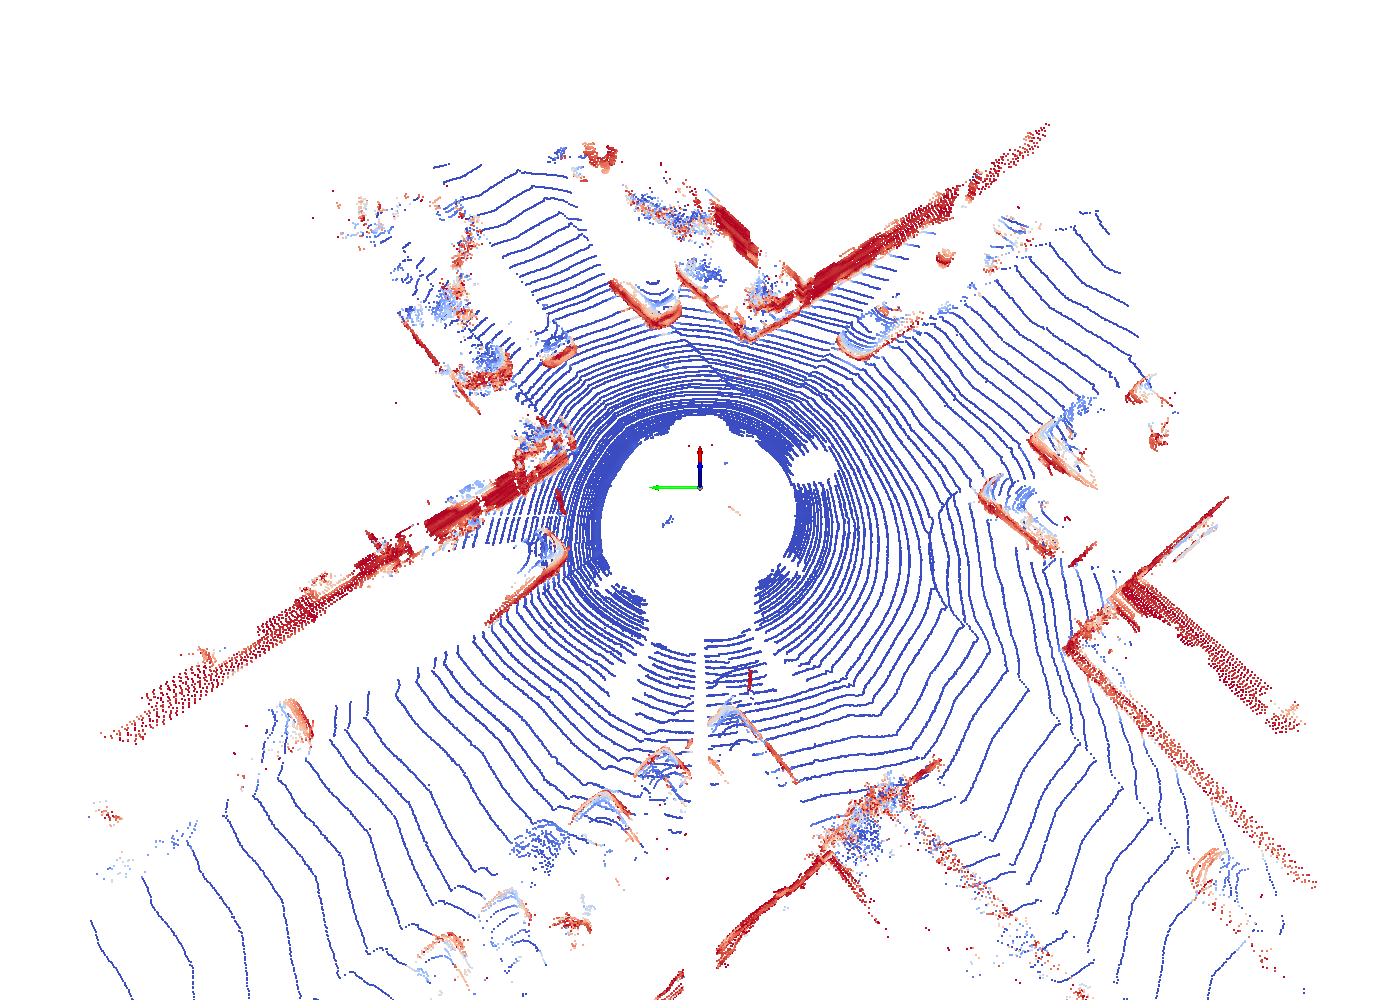
\includegraphics[width=\textwidth]{figures/ej3_verticalidad.png}\caption{Verticalidad: azul horizontal, rojo vertical.}\end{subfigure}
\begin{subfigure}{0.45\textwidth}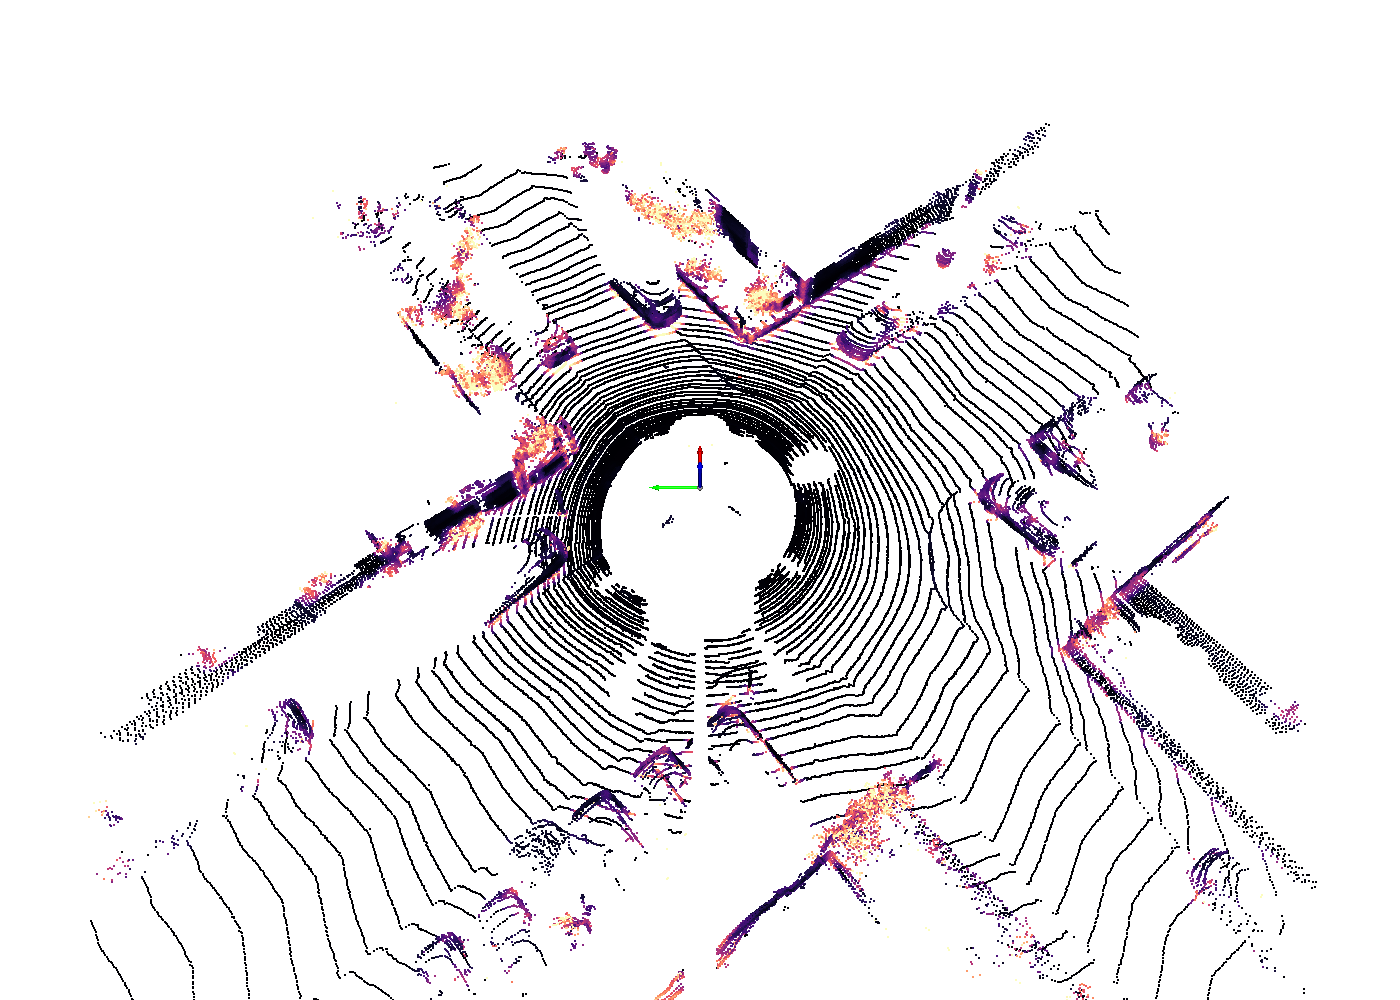
\includegraphics[width=\textwidth]{figures/ej3_curvatura.png}\caption{Curvatura: oscuro liso, claro desordenado.}\end{subfigure}
\caption{Las dos características geométricas del recorte.}
\label{fig:caracteristicas}
\end{figure}

\begin{table}[h]
\centering
\begin{tabular}{lccccc}
\toprule
Atributos de k-means ($k = 2$) & Accuracy & Precision & Recall & F1-score & IoU \\
\midrule
Referencia trivial: todo es suelo & 57{,}1\,\% & 57{,}1\,\% & 100{,}0\,\% & 72{,}7\,\% & 57{,}1\,\% \\
$(x, y, z)$ & 51{,}8\,\% & 61{,}4\,\% & 42{,}5\,\% & 50{,}2\,\% & 33{,}5\,\% \\
$z$ & 85{,}5\,\% & 79{,}8\,\% & 100{,}0\,\% & 88{,}7\,\% & 79{,}8\,\% \\
$z$ + verticalidad + curvatura & 96{,}8\,\% & 95{,}9\,\% & 98{,}6\,\% & 97{,}2\,\% & 94{,}6\,\% \\
\bottomrule
\end{tabular}
\caption{Segmentación del suelo (clase positiva) con k-means, $k = 2$, en el barrido 00/001560.}
\label{tab:suelo}
\end{table}

\begin{tcolorbox}[colback=yellow!8!white, colframe=orange!70!black, title=\textbf{Moraleja}]
El algoritmo era el mismo en los tres casos. k-means no busca ``suelo'' ni ``objetos'': reparte los puntos según su distancia a unos centroides \emph{en el espacio de atributos que le damos}. \textbf{Elegir bien las características importa más que el propio algoritmo.}
\end{tcolorbox}


\section{Objetos con DBSCAN}
Para encontrar objetos, k-means tiene dos problemas: hay que decirle \textbf{cuántos} hay, y sus grupos son siempre ``redondos'' alrededor de un centroide. \textbf{DBSCAN} (\textit{Density-Based Spatial Clustering of Applications with Noise}) agrupa por \textbf{densidad} con dos parámetros: un radio \texttt{eps} y un número mínimo de vecinos \texttt{min\_samples}.
\begin{itemize}
    \item Un punto es \textbf{núcleo} si tiene al menos \texttt{min\_samples} puntos (contándose a sí mismo) a una distancia menor  de \texttt{eps}.
    \item Dos núcleos a una distancia menor de \texttt{eps} se fusionan en el mismo grupo; así, un grupo crece encadenando núcleos y puede tener \textbf{cualquier forma}.
    \item Un punto que no es núcleo pero está una distancia menor de \texttt{eps} de un punto que es \textbf{borde}, se une a su grupo. El resto es \textbf{ruido} (etiqueta $-1$).
\end{itemize}
El número de grupos lo decide el algoritmo. Para que el suelo no una todos los objetos entre sí, primero se quita, y se agrupa en \textbf{vista cenital}, solo con $(x, y)$. Aquí el suelo se quita con las etiquetas, para estudiar DBSCAN por separado; en un coche real se quitaría con un filtro geométrico (un plano ajustado con RANSAC, el filtro CSF\dots) o con un agrupamiento como el del ejercicio~\ref{ej:suelo}. También se quitan los puntos a más de unos 2{,}5\,m de altura (copas de árboles, aleros), que vistos desde arriba unirían lo que tienen debajo. Para medir el resultado, las etiquetas de instancia dicen qué puntos son de cada coche. Se usa el criterio estándar de la segmentación panóptica\footnote{A. Kirillov et al., \textit{Panoptic Segmentation}, CVPR, 2019. Es el criterio del \textit{benchmark} panóptico de SemanticKITTI.}: un coche es \textbf{detectado} si algún grupo tiene con él un $\text{IoU} > 0{,}5$, donde
\[
\text{IoU}(\text{coche}, \text{grupo}) = \frac{|\text{coche} \cap \text{grupo}|}{|\text{coche} \cup \text{grupo}|}
\]
cuenta puntos. Con ese umbral cada coche solo puede emparejarse con un grupo, y, como en SemanticKITTI, se ignoran los coches con menos de 50 puntos. El programa da el \textbf{recall} (coches detectados entre coches que hay) y el \textbf{IoU medio} de los detectados, que dice cuánto se parece cada grupo a su coche.

\begin{exercise}\label{ej:dbscan}
Complete \texttt{agrupar\_dbscan} en \texttt{4\_dbscan\_main.py} usando \texttt{sklearn.cluster.DBSCAN} y ejecute el programa.
\begin{enumerate}
    \item[a)] Con \texttt{eps} $= 0{,}5$\,m y \texttt{min\_samples} $= 8$ sobre los 46\,769 puntos de objeto debe obtener \textbf{45 grupos y 75 puntos de ruido}, con \textbf{15 de los 16 coches} detectados (recall 93{,}8\,\%) y un IoU medio de \textbf{0{,}97}. Busque en \texttt{open3d} el coche que falla, a unos 20\,m del sensor: ¿con qué se ha juntado?
    \item[b)] El programa repite DBSCAN con varios \texttt{eps}: debe ver 98, 66, 45, 25 y 6 grupos para 0{,}2, 0{,}3, 0{,}5, 1 y 2\,m, con un recall de coches del 87{,}5, 100, 93{,}8, 56{,}2 y 6{,}2\,\%. Explique qué ocurre con los objetos cuando \texttt{eps} es demasiado pequeño y cuando es demasiado grande. Con 0{,}3\,m se detectan todos los coches; ¿por qué aun así puede no ser la mejor elección? (Pista: la métrica solo mira los coches; fíjese en el número de grupos y de puntos de ruido.)
    \item[c)] k-means (el suyo) con $k = 45$, el número de grupos de DBSCAN, detecta solo \textbf{10 de 16} coches (recall 62{,}5\,\%), con un IoU medio de \textbf{0{,}80}. Compare en \texttt{open3d} con el apartado a): ¿qué hace k-means con un muro largo? ¿Y con dos coches aparcados muy juntos?
    \item[d)] DBSCAN \textbf{sin quitar el suelo}, en $(x, y, z)$. ¿Qué porcentaje de los puntos acaba en el grupo mayor (90{,}9\,\%)? ¿Por qué?
\end{enumerate}
Opcional: cambie \texttt{BARRIDO} por \texttt{data/kitti\_08\_003880} en los ejercicios 3 y 4. En el ejercicio 3, el F1-score pasa del 71{,}8\,\% con la $z$ sola al 88{,}7\,\% con las características geométricas (la referencia trivial da 55{,}9\,\%). En el 4, DBSCAN detecta 9 de 11 coches (IoU medio 0{,}90) y k-means, 5 (IoU medio 0{,}78).
\end{exercise}

\begin{figure}[h]
\centering
\begin{subfigure}{0.32\textwidth}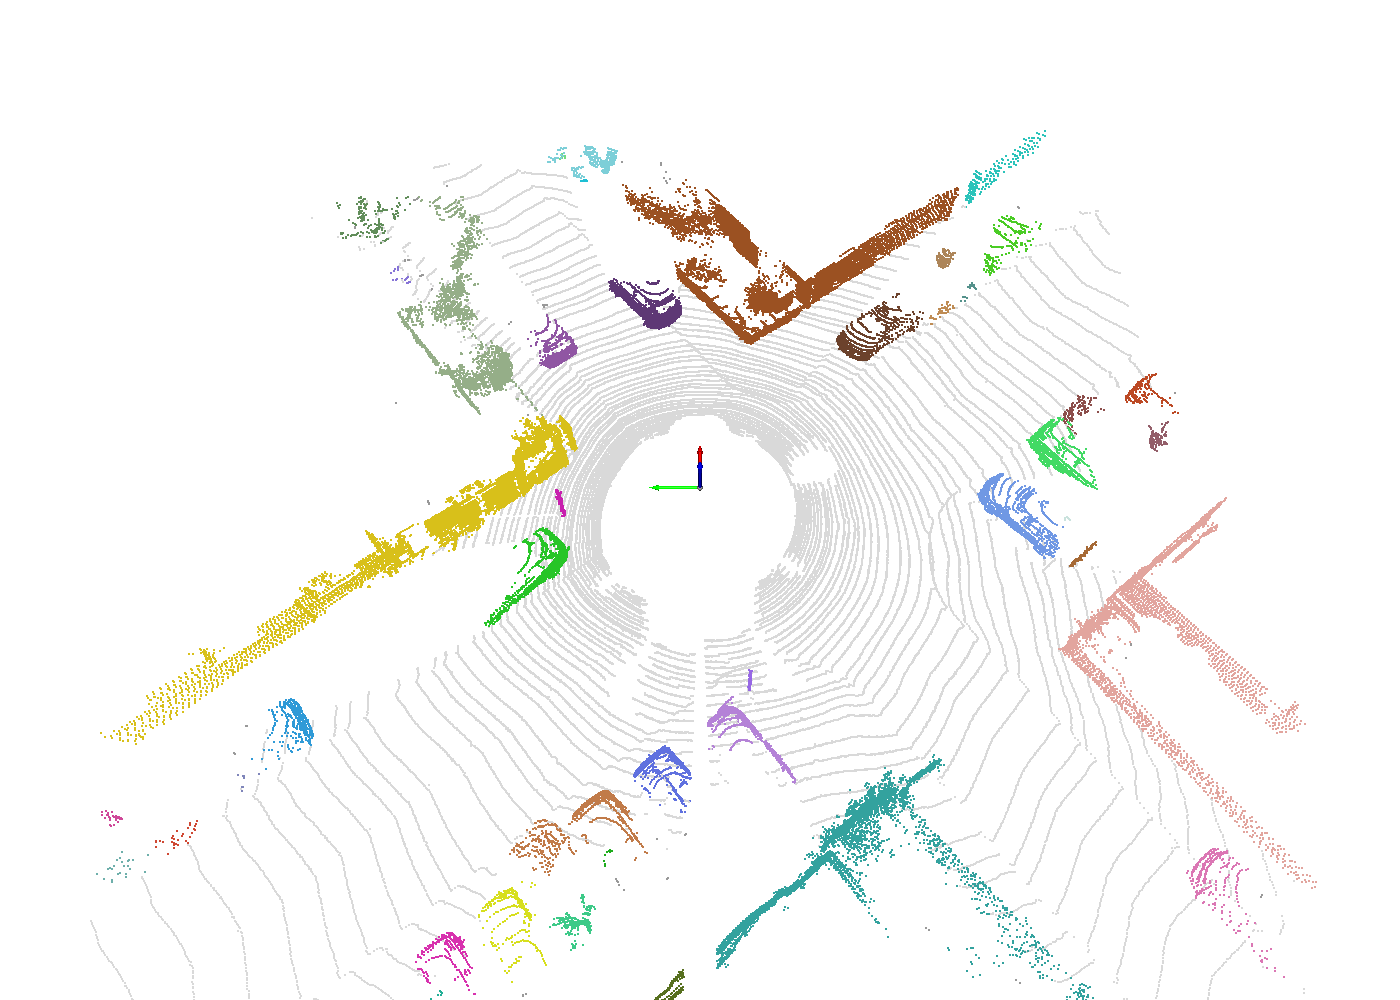
\includegraphics[width=\textwidth]{figures/ej4_dbscan.png}\caption{DBSCAN, 45 grupos.}\end{subfigure}
\begin{subfigure}{0.32\textwidth}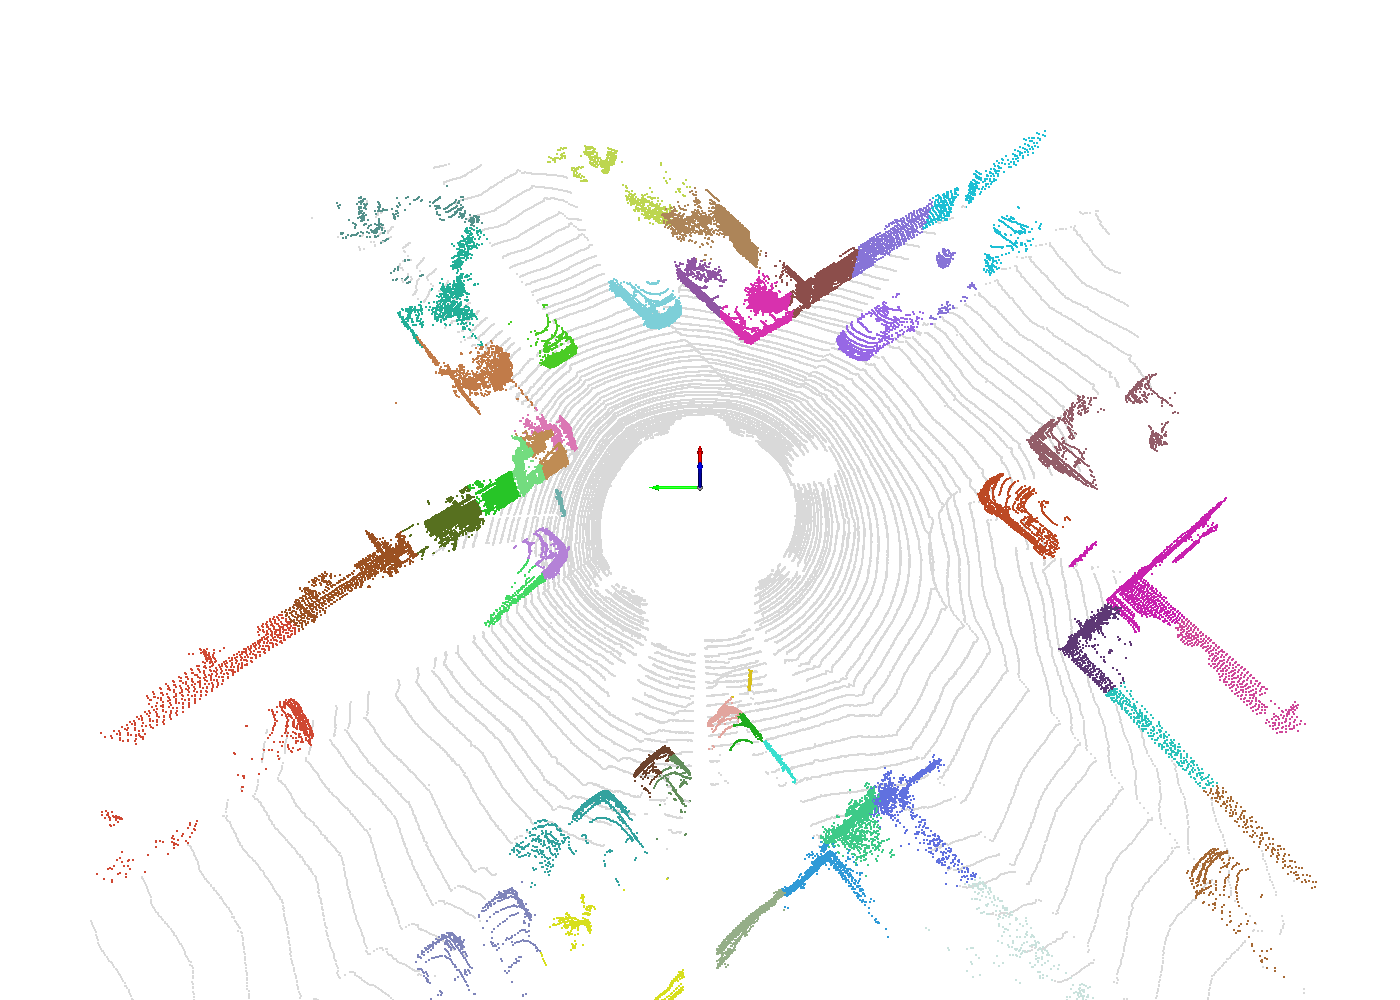
\includegraphics[width=\textwidth]{figures/ej4_kmeans.png}\caption{k-means, $k = 45$.}\end{subfigure}
\begin{subfigure}{0.32\textwidth}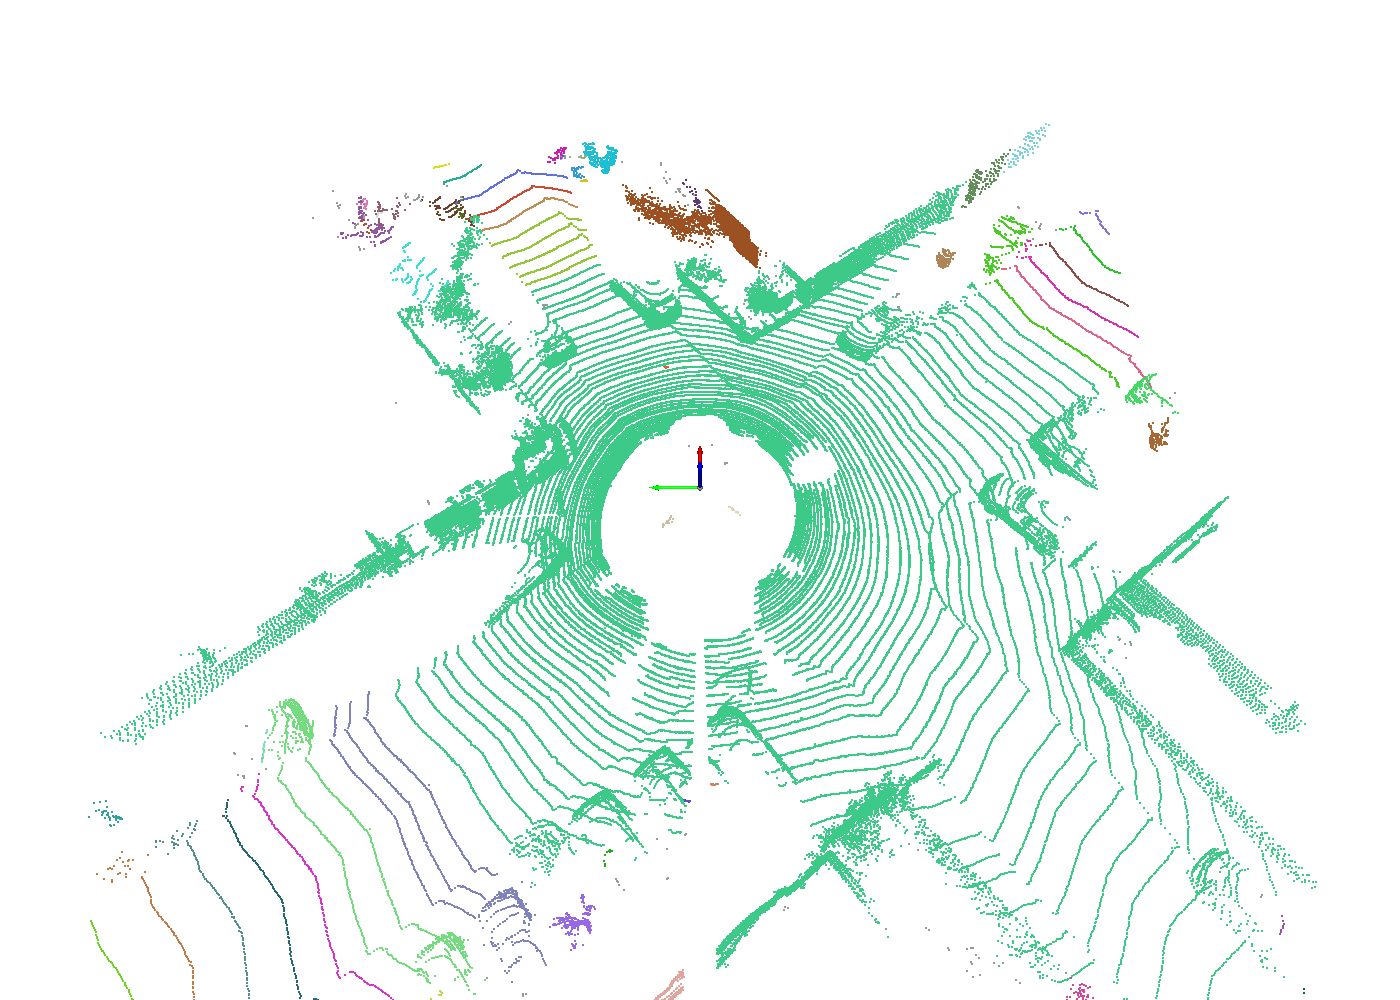
\includegraphics[width=\textwidth]{figures/ej4_dbscan_con_suelo.png}\caption{DBSCAN con el suelo.}\end{subfigure}
\caption{Un color por grupo. En (a) y (b) el suelo, que no se agrupa, aparece en gris claro; en (a) el ruido aparece en gris.}
\label{fig:dbscan}
\end{figure}

\begin{tcolorbox}[colback=yellow!8!white, colframe=orange!70!black, title=\textbf{Para terminar}]
k-means agrupa los puntos por \textbf{cómo son} (sus características: altura, verticalidad, curvatura); DBSCAN, por \textbf{dónde están} (qué puntos se tocan con cuáles). Juntos forman un sistema de percepción completo: primero se separa el suelo de lo demás y después lo demás se trocea en objetos.
\end{tcolorbox}

\end{document}
